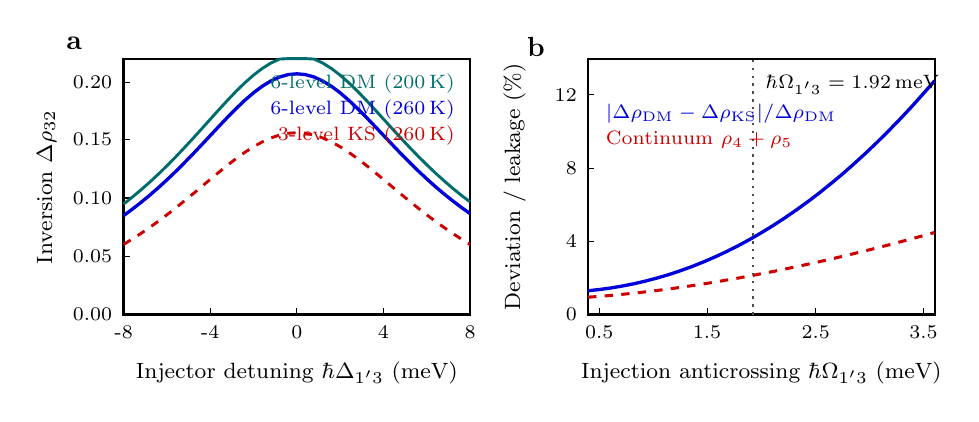
\begin{tikzpicture}[x=1cm,y=1cm,font=\footnotesize]
  % Panel a: Population inversion vs detuning
  \node[anchor=north west,font=\bfseries\normalsize] at (0.10,4.35) {a};
  \draw[thick] (0.95,0.70) rectangle (5.35,3.95);
  \foreach \v/\y in {0.00/0.70, 0.05/1.44, 0.10/2.18, 0.15/2.92, 0.20/3.65} {
    \draw (0.95,\y) -- (1.03,\y);
    \node[left,font=\scriptsize] at (0.93,\y) {\v};
  }
  \foreach \xval/\xpos in {-8/0.95, -4/2.05, 0/3.15, 4/4.25, 8/5.35} {
    \draw (\xpos,0.70) -- (\xpos,0.78);
    \node[below,font=\scriptsize] at (\xpos,0.68) {\xval};
  }
  \node[below,font=\footnotesize] at (3.15,0.22) {Injector detuning $\hbar\Delta_{1'3}$ (meV)};
  \node[rotate=90,above,font=\footnotesize] at (0.22,2.32) {Inversion $\Delta\rho_{32}$};

  \draw[teal!85!black,line width=1.05pt] (0.950,2.103) -- (1.060,2.190) -- (1.170,2.282) -- (1.280,2.379) -- (1.390,2.481) -- (1.500,2.588) -- (1.610,2.700) -- (1.720,2.816) -- (1.830,2.935) -- (1.940,3.056) -- (2.050,3.179) -- (2.160,3.301) -- (2.270,3.421) -- (2.380,3.536) -- (2.490,3.643) -- (2.600,3.740) -- (2.710,3.824) -- (2.820,3.893) -- (2.930,3.944) -- (3.040,3.950) -- (3.150,3.950) -- (3.260,3.950) -- (3.370,3.944) -- (3.480,3.893) -- (3.590,3.824) -- (3.700,3.740) -- (3.810,3.643) -- (3.920,3.537) -- (4.030,3.423) -- (4.140,3.304) -- (4.250,3.183) -- (4.360,3.062) -- (4.470,2.942) -- (4.580,2.825) -- (4.690,2.711) -- (4.800,2.602) -- (4.910,2.497) -- (5.020,2.398) -- (5.130,2.303) -- (5.240,2.214) -- (5.350,2.131);
  \draw[blue!85!black,line width=1.2pt] (0.950,1.956) -- (1.060,2.037) -- (1.170,2.123) -- (1.280,2.214) -- (1.390,2.309) -- (1.500,2.410) -- (1.610,2.515) -- (1.720,2.625) -- (1.830,2.738) -- (1.940,2.854) -- (2.050,2.972) -- (2.160,3.089) -- (2.270,3.205) -- (2.380,3.316) -- (2.490,3.421) -- (2.600,3.516) -- (2.710,3.598) -- (2.820,3.666) -- (2.930,3.716) -- (3.040,3.747) -- (3.150,3.757) -- (3.260,3.747) -- (3.370,3.716) -- (3.480,3.665) -- (3.590,3.598) -- (3.700,3.516) -- (3.810,3.421) -- (3.920,3.317) -- (4.030,3.207) -- (4.140,3.092) -- (4.250,2.976) -- (4.360,2.860) -- (4.470,2.745) -- (4.580,2.634) -- (4.690,2.526) -- (4.800,2.423) -- (4.910,2.324) -- (5.020,2.231) -- (5.130,2.143) -- (5.240,2.060) -- (5.350,1.982);
  \draw[red!80!black,dashed,line width=1.05pt] (0.950,1.590) -- (1.060,1.658) -- (1.170,1.729) -- (1.280,1.805) -- (1.390,1.884) -- (1.500,1.966) -- (1.610,2.052) -- (1.720,2.141) -- (1.830,2.231) -- (1.940,2.323) -- (2.050,2.416) -- (2.160,2.507) -- (2.270,2.596) -- (2.380,2.681) -- (2.490,2.760) -- (2.600,2.831) -- (2.710,2.892) -- (2.820,2.942) -- (2.930,2.979) -- (3.040,3.002) -- (3.150,3.009) -- (3.260,3.002) -- (3.370,2.979) -- (3.480,2.942) -- (3.590,2.892) -- (3.700,2.831) -- (3.810,2.760) -- (3.920,2.681) -- (4.030,2.596) -- (4.140,2.507) -- (4.250,2.416) -- (4.360,2.323) -- (4.470,2.231) -- (4.580,2.141) -- (4.690,2.052) -- (4.800,1.966) -- (4.910,1.884) -- (5.020,1.805) -- (5.130,1.729) -- (5.240,1.658) -- (5.350,1.590);

  \node[anchor=north east,font=\scriptsize,teal!85!black] at (5.28,3.88) {6-level DM ($200\,\mathrm{K}$)};
  \node[anchor=north east,font=\scriptsize,blue!85!black] at (5.28,3.55) {6-level DM ($260\,\mathrm{K}$)};
  \node[anchor=north east,font=\scriptsize,red!80!black] at (5.28,3.22) {3-level KS ($260\,\mathrm{K}$)};

  % Panel b: Relative error & continuum leakage vs Omega_13
  \node[anchor=north west,font=\bfseries\normalsize] at (5.95,4.35) {b};
  \draw[thick] (6.85,0.70) rectangle (11.25,3.95);
  \foreach \v/\y in {0/0.70, 4/1.63, 8/2.56, 12/3.49} {
    \draw (6.85,\y) -- (6.93,\y);
    \node[left,font=\scriptsize] at (6.83,\y) {\v};
  }
  \foreach \xval/\xpos in {0.5/6.99, 1.5/8.36, 2.5/9.74, 3.5/11.11} {
    \draw (\xpos,0.70) -- (\xpos,0.78);
    \node[below,font=\scriptsize] at (\xpos,0.68) {\xval};
  }
  \node[below,font=\footnotesize] at (9.05,0.22) {Injection anticrossing $\hbar\Omega_{1'3}$ (meV)};
  \node[rotate=90,above,font=\footnotesize] at (6.18,2.32) {Deviation / leakage (\%)};

  \draw[blue!85!black,line width=1.2pt] (6.850,1.002) -- (6.997,1.018) -- (7.143,1.038) -- (7.290,1.063) -- (7.437,1.092) -- (7.583,1.126) -- (7.730,1.165) -- (7.877,1.208) -- (8.023,1.257) -- (8.170,1.310) -- (8.317,1.369) -- (8.463,1.432) -- (8.610,1.501) -- (8.757,1.575) -- (8.903,1.654) -- (9.050,1.739) -- (9.197,1.829) -- (9.343,1.924) -- (9.490,2.025) -- (9.637,2.131) -- (9.783,2.242) -- (9.930,2.360) -- (10.077,2.482) -- (10.223,2.611) -- (10.370,2.745) -- (10.517,2.885) -- (10.663,3.030) -- (10.810,3.181) -- (10.957,3.338) -- (11.103,3.501) -- (11.250,3.669);
  \draw[red!80!black,dashed,line width=1.1pt] (6.850,0.920) -- (6.997,0.931) -- (7.143,0.943) -- (7.290,0.957) -- (7.437,0.972) -- (7.583,0.988) -- (7.730,1.006) -- (7.877,1.025) -- (8.023,1.045) -- (8.170,1.067) -- (8.317,1.089) -- (8.463,1.113) -- (8.610,1.138) -- (8.757,1.163) -- (8.903,1.190) -- (9.050,1.218) -- (9.197,1.246) -- (9.343,1.276) -- (9.490,1.307) -- (9.637,1.338) -- (9.783,1.370) -- (9.930,1.404) -- (10.077,1.438) -- (10.223,1.473) -- (10.370,1.509) -- (10.517,1.546) -- (10.663,1.583) -- (10.810,1.622) -- (10.957,1.661) -- (11.103,1.701) -- (11.250,1.742);
  \draw[dotted,black!70,line width=0.85pt] (8.94,0.70) -- (8.94,3.95);
  \node[anchor=north west,font=\scriptsize] at (8.98,3.86) {$\hbar\Omega_{1'3}=1.92\,\mathrm{meV}$};
  \node[anchor=north west,font=\scriptsize,blue!85!black] at (6.95,3.50) {$|\Delta\rho_{\mathrm{DM}}-\Delta\rho_{\mathrm{KS}}|/\Delta\rho_{\mathrm{DM}}$};
  \node[anchor=north west,font=\scriptsize,red!80!black] at (6.95,3.15) {Continuum $\rho_4+\rho_5$};
\end{tikzpicture}
